\documentclass[journal,12pt,onecolumn]{IEEEtran}
\usepackage[cmex10]{amsmath}
\renewcommand\thesection{\arabic{section}}
\usepackage{subfig}
\usepackage{longtable}
\usepackage{tikz}
\usepackage{circuitikz}
\usepackage{longtable}
\usepackage{multirow}
\usepackage{amsthm}
%\usepackage{iithtlc}
\usepackage{mathrsfs}
\usepackage{txfonts}
\usepackage{stfloats}
\usepackage{bm}
\usepackage{cite}
\usepackage{cases}
\usepackage{subfig}
%\usepackage{xtab}
\usepackage{longtable}
\usepackage{multirow}
%\usepackage{algorithm}
%\usepackage{algpseudocode}
\usepackage{enumitem}
\usepackage{mathtools}
\usepackage{steinmetz}
\usepackage{tikz}
\usepackage{circuitikz}
\usepackage{verbatim}
\usepackage{tfrupee}
\usepackage[breaklinks=true]{hyperref}
%\usepackage{stmaryrd}
\usepackage{tkz-euclide} % loads  TikZ and tkz-base
%\usetkzobj{all}
\usetikzlibrary{calc,math}
\usepackage{listings}
\usepackage{color}                                            %%
\usepackage{array}                                            %%
\usepackage{longtable}                                        %%
\usepackage{calc}                                             %%
\usepackage{multirow}                                         %%
\usepackage{hhline}                                           %%
\usepackage{ifthen}                                           %%
%optionally (for landscape tables embedded in another document): %%
\usepackage{lscape}     
\usepackage{multicol}
\usepackage{chngcntr}
\hyphenation{op-tical net-works semi-conduc-tor}
\def\inputGnumericTable{}                                 %%

\lstset{
	%language=C,
	frame=single, 
	breaklines=true,
	columns=fullflexible
}
%\lstset{
%language=tex,
%frame=single, 
%breaklines=true
%}
\begin{document}
\title{Friquency Offset Estimation}
\maketitle
\section{Maximum likelyhood mathod}
\begin{enumerate}
	\item In a multicarrier  system  there is a dissimilarity of the oscillators used at the transmitter and receiver which  causes a ofset in the carrier friquency.Due to this at the receiver end when the signal is demodulated, we get a very high bit rate error.
	
	To overcome this eror ML stimation is used and ML carrier frequency estimater 
	\begin{align}
	\triangle f &= \frac{1}{2\pi T_s}\frac{\sum_{k=1}^{M} Im{R(k)}}{\sum_{k=1}^{M} kRe{R(k)}}
	\end{align}
	
	Where the  $\triangle$f is the frquency  offset$T_s$ is the sampeling interval.
	
	\item R(k) denotes the estimated autocorrelation of the sequence $r_k$.
	
	\begin{align}
	R(k) &= \frac{1}{N-K}{\sum_{i = k+1}^{M} r_ir_{i-k}^*}	
	\end{align}
	$r_k $is the sampled signal which can be represnted as $\to$
	\begin{align}
	r_k &= e^{j2\pi \triangle fT_s + \theta}	+ v_k
	\end{align}
	$1\leq k \leq N$
	\\
	$v_k$ is the compex noise.
	\\
   \begin{align}
    \sum_{k=1}^{M} Im{R(k)} = M arg{\sum_{k=1}^{M} {R(k)}}
    \\
    \sum_{k=1}^{M} kRe{R(k)} = M\frac{M+1}{2}
	\end{align}
	\item Thus total no of the quation used are 5.
\end{enumerate}

\section{Simulation for frequency estimation}

	 Simulation shows that symbols with a constant offset frequency are transferred through a wirless comunication channel.At the receiver end this offset frequency is estimated with the ML mwthode.Process is repated for the different value of the signal's amplitude A.
	
	In ML estimation $r_k$ is the received signal and R(k) represents the autocorelation of the  $r_k$. If the length of the incomming signal is N then R(k)will be $\to$
	\\
	\begin{align}
		{\sum_{i = k+1}^{M} r_ir_{i-k}^*}
	\end{align}
	\\
	When the value of the k is near to the N then it gives a poor estimate of the autocorilation of $r_k$ so we use values of k lower than N to discard the unrelible autocorrelation estimates.Using the taylor series expansion of the frequency estimator we  aproximate  and get the final equation as$\to$ 
	\\
	\begin{align}
	\triangle f &= \frac{1}{2\pi T_s}\frac{\sum_{k=1}^{M} Im{R(k)}}{\sum_{k=1}^{M} kRe{R(k)}}
	\end{align}	

\section{Observation}

	
	For different value of m and for fix length of simlen simulaton is performed.From $m =5$ to $m= 50$ is taken for  different graphs where simlen is 50 and frequency is 50K.

\begin{figure}[!ht]
	\centering
	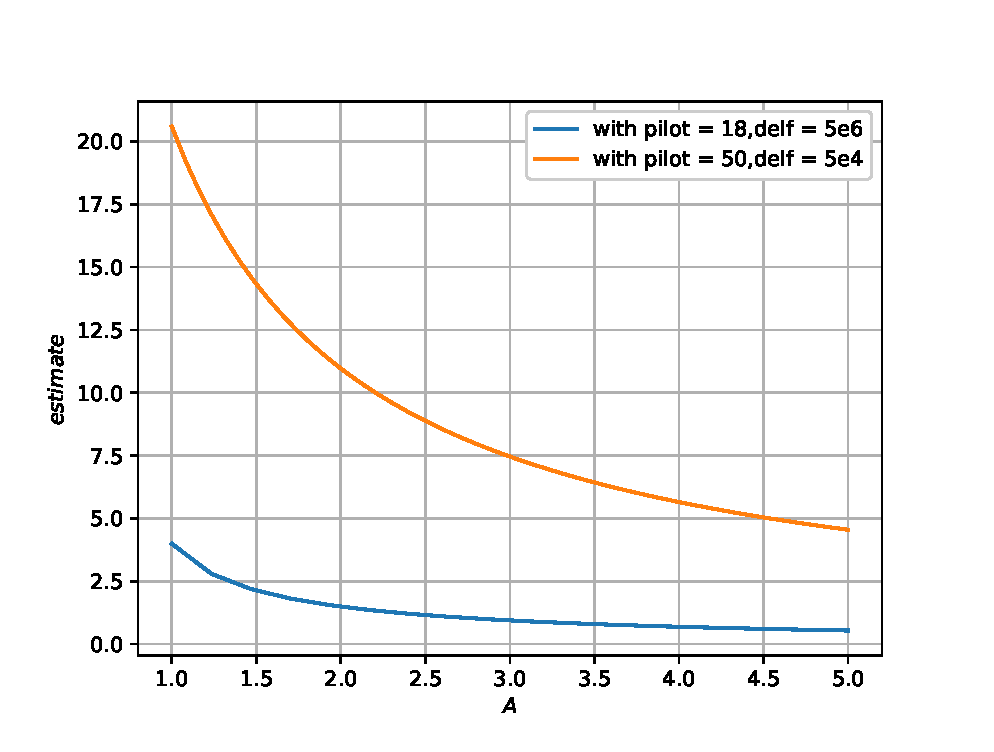
\includegraphics[width=0.5\columnwidth]{./comparision/frequency.eps}
	\caption{comaprision of graph of offset friquency for different M }
	\label{fig:offset frequency}
\end{figure}
table for the variables and values used in the code
\begin{table}[!ht]
%	\centering
	\input{./Frequency.tex}
	\caption{List of variable }
\end{table}

\section{Conclusion}
	 In this simulation frequency and simlen is constant and M varies from 5 to 50. For  m$\leq$10  the value of  estimate variable  varies from 10 to 400 and everage is 120 for A = 1 as shown in graph. For m$\geq$10  the value of the estimate variable  varies from 0.2 to 70 and average is 35 for A = 1.thus in short we can say that for the smaler value of M error is large than that of for larger M.

\end{document}